\chapter{Results and Analysis}
\label{chp:results}
\section{Survey results}
\label{chp:surveyResults}
Looking at the survey results where there was a total of 27 respondents, we can see that our algorithm was preferred $\frac{2}{3}$ of the times, as can be seen in figure \ref{fig:surveyOverall}. This indicates that our algorithm is more suitable for finding highlights for certain types of players. Most of the respondents were very familiar with the game, showing that experienced players seemed to like our implementation.
\begin{figure}
\centering
\begin{tikzpicture}[object/.style={thin,double,<->}]
 \pie{66.6/Our algorithm,33.3/Allstar}
\end{tikzpicture}
\caption{Pie chart showing what algorithm won in the survey}
\label{fig:surveyOverall}
\end{figure}

\begin{table}[]
\begin{tabular}{|l|l|l|l|}
\hline
Match & Our Algorithm & Allstar & Indifferent \\ \hline
1     & 40,7\%        & 37\%    & 22.3\%      \\ \hline
2     & 33.3\%        & 55.6\%  & 11.1\%      \\ \hline
3     & 63\%          & 22.2\%  & 14.8\%      \\ \hline
4     & 48.2\%        & 44.4\%  & 7.4\%       \\ \hline
5     & 59.3\%        & 33.3\%  & 7.4\%       \\ \hline
6     & 40.8\%        & 44.4\%  & 14.8\%      \\ \hline
7     & 48.2\%        & 37\%    & 14.8\%      \\ \hline
8     & 66.7\%        & 25.9\%  & 7.4\%       \\ \hline
9     & 25.9\%        & 59.3\%  & 14.8\%      \\ \hline
\end{tabular}
\end{table}
\subsection*{Match 1}
For this set of highlights, video A was got more votes by a slim margin. The people who taught video A was the better one commented that it was more tactical and \gls{clean}. That the AK47 was used instead of the Glock also attracted some viewers. One respondent said; "It was a good clutch". The respondents who liked video B had the opinion that the highlight had more action. The people who responded indifferently mentioned that both clips were the same in terms of level of gameplay.

\subsection*{Match 2}
For this set of highlights, video B had more votes, with a little more than half of the respondents liking this highlight more. Respondents mentioned that the knife kill during video B was a large factor, and that the kills were all solo plays, with no help from teammates. They also mentioned that video A was more messy and video B was more clean.

\subsection*{Match 3}
For this set of highlights, Video B was the preferred highlight. While several viewers liked the impressive 4K spray down and first kills in Video A, the majority found the gameplay in Video B to be better.

Some comments highlighted specific reasons why Video B was more appealing.

\begin{itemize}
\item \textbf{Better decision-making:} One respondent said that "The Read on The Game is on the 2nd Video way more accurate."
\item \textbf{Map awareness:} Another respondent said "Better checks on corners."
\item \textbf{Overall gameplay:} Several viewers simply stated their preference for Video B, indicating a more enjoyable viewing experience.
\end{itemize}

\subsection*{Match 4}


For this set of highlights, Video B was the preferred highlight for a few reasons.

\begin{itemize}
\item \textbf{Fast-paced action:} One respondent stated, "Video B was way fast-paced, which I like more."
\item \textbf{Strategic gameplay:} One respondent commented: "Just a better round, he knows what he is doing and plays around the enemies making mistakes" which shows a more calculated approach to the game.
\item \textbf{Map control:} Another viewer noted that "Video B felt like it opened up an A push pretty cleanly," showing that taking initiative and opening up a site makes a good highlight.
\end{itemize}

Overall, viewers found Video B to be a better highlight, due to its faster and more strategic gameplay. The criticism of Video A mentioned a hesitation to push forward, and some bad mechanics regarding jump spotting.
\subsection*{Match 5}
People liked Video B more in this set of highlights.
The reasons that the respondents liked video B more:

\begin{itemize}
\item \textbf{Used smoke well:} "Played the smoke (very nice!) on video B"
\item \textbf{Got more kills:} "In video B he does not die, and gets most of the kills"
\item \textbf{Won the round:} "He didnt die, and won round"
\end{itemize}

While some people liked the skills shown in Video A, most preferred Video B because the player made good choices and won their team the round, as well as he did not die.


\subsection*{Match 6}

Most people liked Video B more, saying it had cleaner kills. Some people liked Video A because it was fast-paced and showed teamwork.

The difference between the highlights were:
\begin{itemize}
\item \textbf{Video A - Fast and teamwork:} Some respondents liked how Video A was quicker and showed the whole team working together.
\item \textbf{Video B - Cleaner kills:} Others thought the kills in Video B looked nicer and smoother.
\end{itemize}

A few respondents said both videos were good and bad in different ways. Some also mentioned the team kills during that round.



\subsection*{Match 7}
The survey results show that people liked Video A more. Video A had more kills, including a cool 2-kill spray down, and the player got the last kill. Some people also liked that it was faster-paced.

\begin{itemize}
\item \textbf{More kills and a cool spray:} "More kills, aswell as a nice 2K spraydown."
\item \textbf{Got the last kill:} "He made the last kill himself in Video A liked that better."
\item \textbf{Faster pace:} "it was also way more fast paced."
\end{itemize}

Some people liked Video B and thought the player made smarter choices, but overall, Video A was more popular.


\subsection*{Match 8}
The survey shows that video A was the preferred highlight, particularly for the clutch situation, cleaner kills, and higher kill count. While Video B was liked for its efficient 3K, some respondents noted the opponent's missed AWP shots as a huge reason that the highlight even was possible.

\begin{itemize}
\item \textbf{Video A's clutch and kills:} Several viewers favored Video A for the player's ability to secure kills in a clutch situation and the overall higher kill count.
\item \textbf{Video A's cleaner kills:} Some viewers specifically mentioned that the kills in Video A were cleaner and more impressive.
\item \textbf{Video B's methodical 3K:} While acknowledging the skill involved in the 3K in Video B, viewers also pointed out the opponent's missed AWP shots were the only reason this highlight was possible.
\end{itemize}

Overall, the respondents liked Video A for its clutch, and higher kill count and overall was cleaner and Video B was liked for its systematic approach even tho some luck was involved.


\subsection*{Match 9}
Video B won here due to its better game sense, and that it was fast-paced. The highlight was long and showed that it took a long time for the player to win the round.
The reasoning given by the respondents was:

\begin{itemize}
\item \textbf{Video B's better kills:} Multiple viewers highlighted Video B's better kills, with one specifically mentioning the "clean glock 2K."
\item \textbf{Fast-paced action:} Viewers enjoyed the fast pace of Video B, particularly the initial kills.
\end{itemize}



\section{How can one create an algorithm to find better highlights in Counter Strike 2}
The first thing one needs to do is to figure out what metrics should be included in the algorithm. Here, you could interview people in the scene with experience, like casters, analysts, and players of the game. You can also study popular highlights from the community, and see what metrics are the highest in the highlights you watched, and use that as a baseline for what metrics are important to include in highlights. 

The next step in the process of creating an algorithm for highlights is to extract the data. Here there are a few approaches that you can take. There is the approach that we took, which is implementing a parser step, to extract all relevant data from the demo file, and gives it into a workable format for the algorithm. Another way to do this is to analyze the video feed from either a screen capture or from a video file. This would require looking at properties of the video / stream, for example watching the kill feed or chat with OCR, and extract data from that, as well as other game information from the UI. Another approach is to use Counter Strike game state integration \footnote{\url{https://developer.valvesoftware.com/wiki/Counter-Strike:_Global_Offensive_Game_State_Integration}} to get the data in real time from the game itself during the match. This would allow taking a clip of the user screen instead of having to render the clip on a separate server. The game state integration provides much the same data as a demo file would but in real time.

Once the data has been collected, you would need to analyze that somehow. This is the most "free" part. Depending on what you want to include in the highlights, this will differ a lot. In our case, we focused on mechanical plays, like kills and the skill of the player, but another way would be to focus on funny plays.

Once this is done, the last part is to output the round number of the highlight, and what player did the highlight. Processing this and rendering the highlight is outside the scope of this algorithm.
\section{What metrics are most important when developing an algorithm to find highlights in Counter Strike 2}

To find what metrics are important for Counter-Strike 2 highlights, we conducted interviews. In these interviews, we got different results. When asked what experience the interviewee had with Counter-Strike or other FPS games 2 out of the 7 had little to no experience with the game Counter-Strike, but 6 out of 7 had played similar games. When asked about experience with highlights in FPS games 2 out of the 7 interviewees had no experience with highlights from FPS games. The 2 that had no little experience with Counter-Strike or other FPS games were the same that had little experience with highlights.\\\\
When asked about their opinion of the most memorable highlight in Counter-Strike history, 6 out of the 7 interviewees answered this question and 4 gave an example of a highlight that could be found on sites like YouTube. One answer was "Yes absolutely. After all, I have both famous ones from big tournaments or matches like Coldzera when he jumps and shoots on Mirage."(Participant L1, personal communication, April 10, 2024). The interviewee that did not give an answer had little to no experience with Counter-Strike.\\\\
When asked about what made it memorable, the interviewees that gave a highlight that could be traced said that things such as casters, personal reference and big stakes. When asked about what makes a good highlight, all interviewees answered. The summary of this:
\begin{itemize}
    \item Winning with odds stacked against you
    \item A demonstration of skill such as \gls{crosshair} placement and movement
    \item Technical skill
    \item Quantity of kills
    \item Short time between kills
    \item Difficult weapon used
    \item 1 vs X situations (one person left on one team while facing x amount of opponents)
    \item Amount of people watching
\end{itemize}
Next the interviewees were asked to rate metrics from 1-10 over the importance the metric had in a highlight. 
In the figure 4.2 each individual rating of the metrics has been collected.
    \begin{figure}[H]
        \centering
        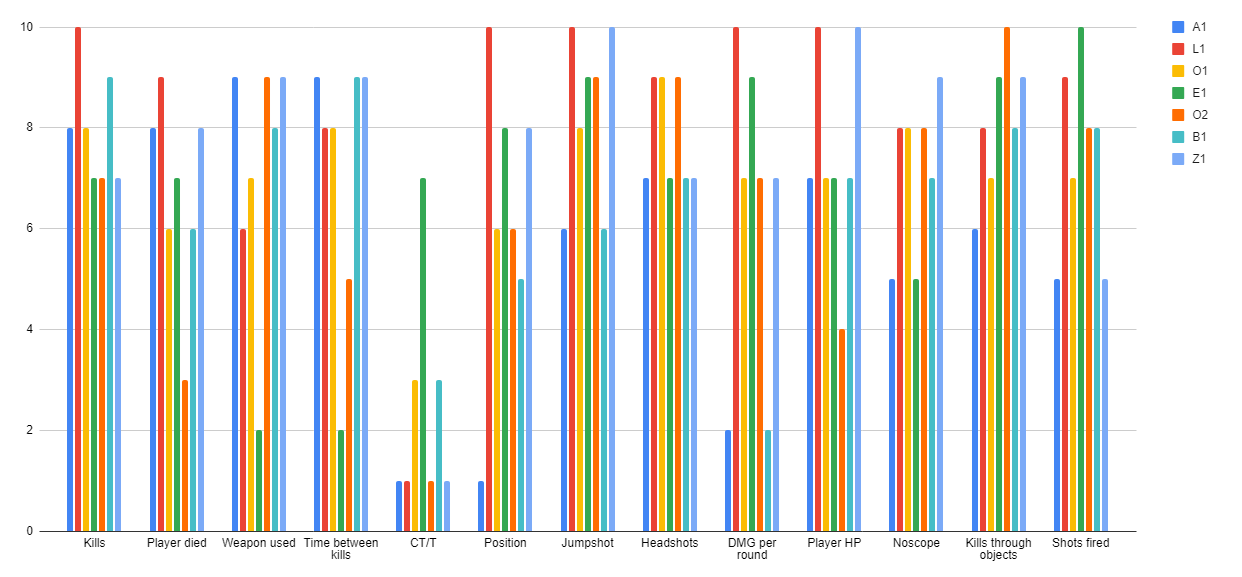
\includegraphics[width=17cm]{Images/All_results.png}
        \caption{Results from metrics rating}
        \label{fig:Barchart}
    \end{figure}
In figure 4.3 we can see the outliers in the answers via the help of box plots. 
    \begin{figure}[H]
        \centering
        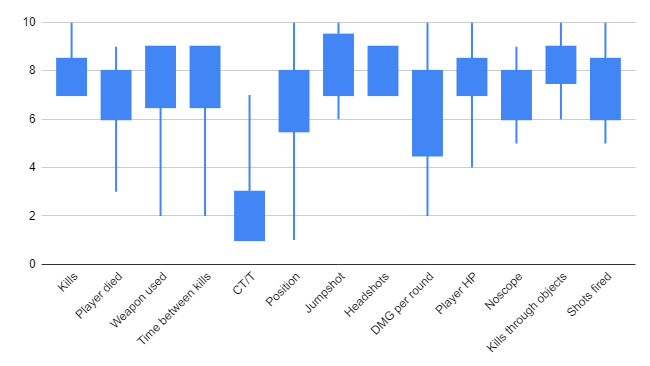
\includegraphics[width=17cm]{Images/boxplot.png}
        \caption{Box plot metrics}
        \label{fig:BoxplotMetrics}
    \end{figure}
    \begin{figure}[H]
        \centering
       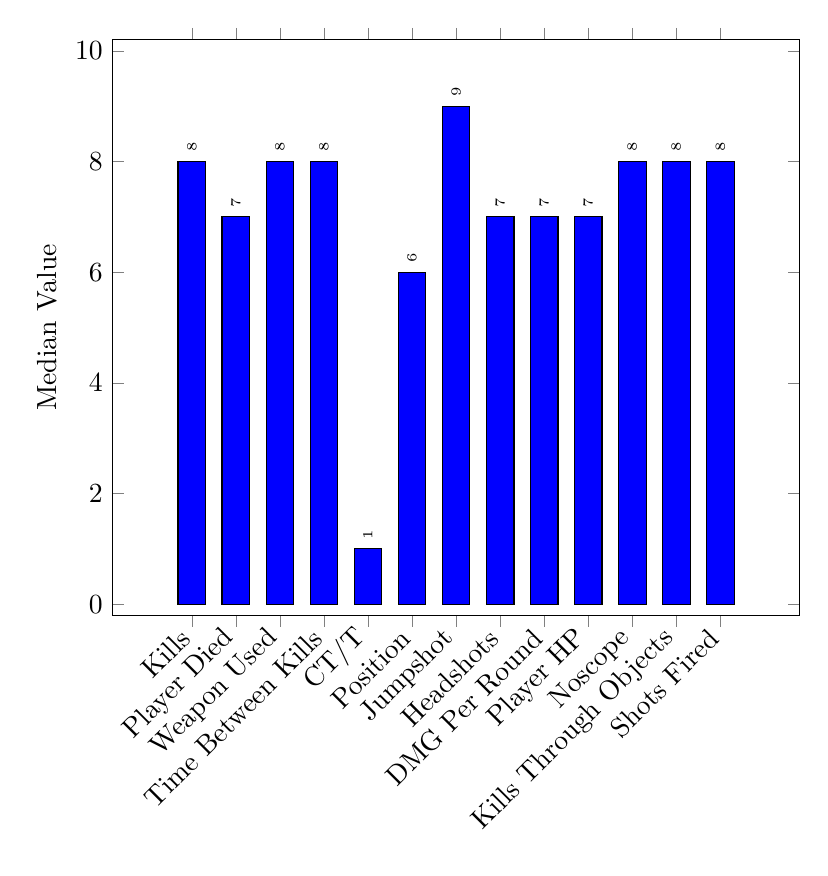
\begin{tikzpicture}


\begin{axis}[
    ybar,
     width=0.85\textwidth,
    bar width=10pt,
    enlargelimits=0.15,
    ylabel={Median Value},
    symbolic x coords={Kills, Player Died, Weapon Used, Time Between Kills, CT/T, Position, Jumpshot, Headshots, DMG Per Round, Player HP, Noscope, Kills Through Objects, Shots Fired},
    xtick=data,
    x tick label style={rotate=45, anchor=east}, 
    nodes near coords,
    every node near coord/.append style={font=\tiny, rotate=90, anchor=west}, 
]

\addplot[fill=blue] coordinates {
    (Kills, 8)
    (Player Died, 7)
    (Weapon Used, 8)
    (Time Between Kills, 8)
    (CT/T,1)
    (Position, 6)
    (Jumpshot, 9)
    (Headshots, 7)
    (DMG Per Round, 7)
    (Player HP, 7)
    (Noscope, 8)
    (Kills Through Objects, 8)
    (Shots Fired, 8)
    % ... (Add other data points here)
};

\end{axis}
\end{tikzpicture}
\caption{Median of metrics}
\label{fig:medianMetrics}
\end{figure}
In figure 4.4 the median value of each metric is displayed which will be used in the algorithm weights.\\\\

When asked about different metrics that we had missed 4 out of the 7 interviewees, all having experience with Counter-Strike, answered with:
\begin{itemize}
    \item Enemy proximity
    \item Hit percentage
    \item \gls{Movement}
    \item \gls{Boosts}
\end{itemize}
When asked if the interviewees used any tools to create highlights, 6 out of 7 interviewees had used a tool to create highlights before. The 1 who had not used any was the interviewee, with little to no experience with highlights and Counter-Strike. The tools used were:
\begin{itemize}
    \item \gls{Faceit}, who provides a highlight if the player gets more or 3 kills
    \item \gls{Esportal}, uses Allstars highlight service
    \item \gls{Leetify}, uses Allstars highlight service
    \item \gls{Medal}, self clipping
    \item \gls{GeForce Experience}, allows users to clip the last 30 seconds or more
    \item \gls{Gifyourgame}, is not supported for Counter-Strike
\end{itemize}
\section{How do the perception of what makes a good highlight differ between novice and experienced players}
In the interviews, the biggest difference between novice and experienced players was in the specificity of the answers, those with less experience had a harder time explaining what they liked in a highlight. There were also fewer real-life examples of highlights from those who had less experience. The rating of metrics was indistinguishable between novice and experienced players, with an outlier of the team side you played which a novice player picked a 7 in importance while the second highest was a 3.\\\\
\begin{figure}[!h]
\centering
\begin{tikzpicture}[object/.style={thin,double,<->}]
 \pie{65.4/Very familiar, 26.9/Somewhat familiar, 7.7/Not Familiar at all}
\end{tikzpicture}
\caption{Pie chart showing experience of Counter-Strike 2}
\label{fig:surveyOverallExperience}
\end{figure}
\\\\
In the surveys, we had a total of 27 participants, with 2 participants who were not familiar at all with Counter-Strike 2, 7 participants that were somewhat familiar with Counter-Strike 2, 17 who were very familiar with Counter-Strike 2 and 1 participant did not answer this question.

The first person mentioned in Match 1 that they liked that video b had more action in it, than video A. Video A consists largely of the player stand around and playing his spot until he decides to get and help out his team. This shows that some less familiar players like the action that you can see, and might not understand the deeper tactics of the game. None of the players left a comment on Match 8 but preferred Video A, where the players goes onto the bombsite. However, in video B, the player runs back and forth, tricking the enemy that he had gone back to another bombsite. This video won, but the less familiar players choose Video A, since they might not see the tactics at play, and that he faked out his enemy.

The other respondent that said they were not familiar with the game said that they liked video A for its clutch, however, since they knew the terminology, they might be still somewhat familiar with the game, showing that people that have played the game appreciate the clutch and smart plays. This respondent did prefer Video A in match 8, so might just prefer the higher speed of the game in Video A.

